\documentclass{article}

\usepackage{amsmath}
\usepackage{amssymb}
\usepackage{amsfonts}
\usepackage{mathtools}

\usepackage[thmmarks, amsmath]{ntheorem}

\usepackage{graphicx}
\usepackage{float}

\usepackage{diffcoeff}
\diffdef{}{op-symbol=\mathrm{d},op-order-sep=0mu}

\usepackage{cancel}
\usepackage{interval}

\usepackage{array}

\usepackage{enumitem}

\setlist[enumerate,1]{label=(\alph*)}

\title{Algebraic Topology Homework 2}
\author{Duarte Maia}
%\date{}

\theoremstyle{plain}
\theorembodyfont{\upshape}
\theoremseparator{.}
\newtheorem{theorem}{Theorem}
\newtheorem{prop}{Prop}
\renewtheorem*{prop*}{Prop}
\newtheorem{lemma}{Lemma}
\newtheorem*{ex}{Exercise}

\theoremstyle{nonumberplain}
\theoremheaderfont{\itshape}
\theorembodyfont{\upshape}
\theoremseparator{:}
\theoremsymbol{\ensuremath{\blacksquare}}
\newtheorem{proof}{Proof}
\newtheorem{sol}{Solution}

\theoremsymbol{\text{\textit{(End proof of lemma)}}}
\newtheorem{lemmaproof}{Proof of lemma}

\newcommand{\R}{\mathbb{R}}
\newcommand{\C}{\mathbb{C}}
\newcommand{\Z}{\mathbb{Z}}
\newcommand{\Q}{\mathbb{Q}}

\newcommand{\kk}{\Bbbk}

\newcommand{\PP}{\mathbb{P}}
\newcommand{\FF}{\mathcal{F}}

\newcommand{\I}{\mathrm{i}}
\newcommand{\e}{\mathrm{e}}

\newcommand{\id}{\mathrm{id}}

\newcommand{\conj}[1]{\overline{#1}}

\DeclareMathOperator{\inte}{int}
\DeclareMathOperator{\codim}{codim}
\newcommand{\grad}{\nabla}


\DeclareMathOperator{\spec}{spec}

\DeclarePairedDelimiter{\abs}{\lvert}{\rvert}
\DeclarePairedDelimiter{\norm}{\lvert}{\rvert}
\DeclarePairedDelimiter{\Norm}{\lVert}{\rVert}
\DeclarePairedDelimiter{\braket}{\langle}{\rangle}


\begin{document}
\maketitle

\begin{ex}[1.2:9]
Show that $M'_h$ does not retract onto $C$, and hence $M_g$ does not retract onto $C$. Show that $M_g$ does retract onto $C'$.
\end{ex}

\begin{sol}
We begin by computing the fundamental group of $M'_h$, using some point $p \in C$ as a basepoint.

To do so, we recall that $M_h$ may be represented as a quotient of a $4h$-gon, with its $4h$ faces identified in a certain way. I don't have to write the details out because they can be found in Hatcher, page 5 of chapter 0.

Now, $M'_h$ may be obtained by removing an open disk $M_h$. Pictorially, it is obvious that we can assume that the removed disk is small, and in this case it is clear that we may shuffle it around a bit (this can be made precise using a local topological chart). Thus, we may assume that the removed disk is found in the interior of the $4h$-gon. While we're at it, we may as well assume that it is the center of the polygon, as it is evident that we may move the puncture inside it without changing the figure up to homeomorphism. Thus, we have a picture like the following. (This picture is for $h = 3$, but it evidently generalizes.)
\begin{figure}[H]
\centering
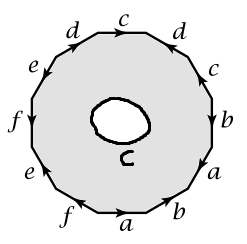
\includegraphics{mph1}
\end{figure}

Now, it is evident that this figure deformation retracts to just its border, which is a wedge of $2h$ circles. Thus, we conclude that the fundamental group of $M'_h$ (with basepoint equal to the vertex, say) is the free group on $2h$ generators, with each edge in the $1$-skeleton of the CW representation of $M_h$ being a generator.

Now, let us look at the following element of $\pi(M'_h)$ (with basepoint equal to the vertex $p$). Go in a straight line from $p$ to the edge of $C$, then follow $C$ clockwise, say, for one full rotation. Then return to $p$ following the reverse of the path previously taken. Call this path $\gamma$.

Then, by homotoping $\gamma$ to the edge of the polygon by a straight-line homotopy, it is easy to see that $[\gamma] \in \pi(M'_h)$ is a product of the generators of $\pi(M'_h)$ in some order, which is not relevant, but crucially, \emph{each generator appears twice in this expression, once with exponent $1$ and once with exponent $-1$}.

Now, suppose that there were a retraction $r \colon M'_h$ to $C$. Then, let us look at $r_*(\gamma)$. If we look at it directly, it is a path that starts in $r(p)$, does some things, does a full rotation, then undoes the things it did at the start. This is a conjugation of a noncontractible path, and hence is noncontractible itself. On the other hand, if we decompose $\gamma$ as a product of generators of $\pi(M'_h, p)$, we see that $r_*(\gamma)$ should be written as a product of a bunch of terms, each of which appears twice, one of which is inverted. Now, since the fundamental product of $C$, a circle, is abelian, this means that $r_*(\gamma)$ must be zero, a contradiction! This proves that such an $r$ may not exist.

\smallskip

This proves that $M_g$ does not retract onto $C$ because if it did, we could restrict such a retraction to $M'_h$.

\medskip

To show that $M_g$ retracts to $C'$, we build such a retraction. To do so, embed $M_g$ into $\R^3$ as in the following figure and separate it into `inside parts', call these $A$, and `outside parts', call them $B$, colored respectively in blue and orange.
\begin{figure}[H]
\centering
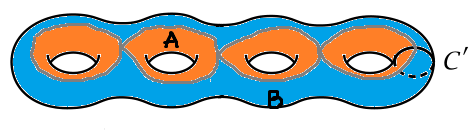
\includegraphics{mph2}
\end{figure}

Note: the gray parts (which represent the border) consist precisely of the points of the surface that maximize and minimize the $z$ coordinate in this embedding.

With this decomposition, we build the retraction as follows. Given a point in the curve, if it is in $A$, there is exactly one set in $C' \cap A$ with the same $z$ coordinate. Define its image under $r$ to be this point. Likewise for $B$.

This map is continuous by the pasting lemma. Indeed, restricted to either $A$ or $B$, it coincides with horizontal projection on a half-circumference, which is continuous, and on the points of $A \cap B$ this definition agrees whether we see the points as points of $A$ or points of $B$. Thus, by the pasting lemma, the resulting map is a continuous map from $M_g$ to $C'$.

Of course, this map fixes all points of $C'$ effectively by definition.
\end{sol}

\begin{ex}[1.2:22]
\leavevmode
\begin{enumerate}
\item Show that $\pi(\R^3 \setminus K)$ has a presentation with one generator $x_i$ for each strip $R_i$ and one relation of the form $x_i x_j x_i^{-1} = x_k$ for each square $S_\ell$.
\item Show that the abelianization of the fundamental group of the complement of a knot is $\Z$.
\end{enumerate}
\end{ex}

\begin{sol}
\leavevmode
\begin{enumerate}
\item We apply the van Kampen theorem to the following decomposition of $X$. Let $A = T \cup R$, where $T$ is the tabletop and $R$ is the union of the (open) rectangles $R_i$, and let $B = T \cup S$, where $S$ consists of a small enough neighborhood of the union of the squares $S_i$; the meaning of `small enough' is made clear in the following figure\footnote{Actually, there is a thing that the figure does not show, which is that $S$ should also be bleeding a bit into the rectangle $R$ under $S$.}, which represents $A$, $B$, and $A \cap B$ in a neighborhood of a crossing.
\begin{figure}[H]
\centering
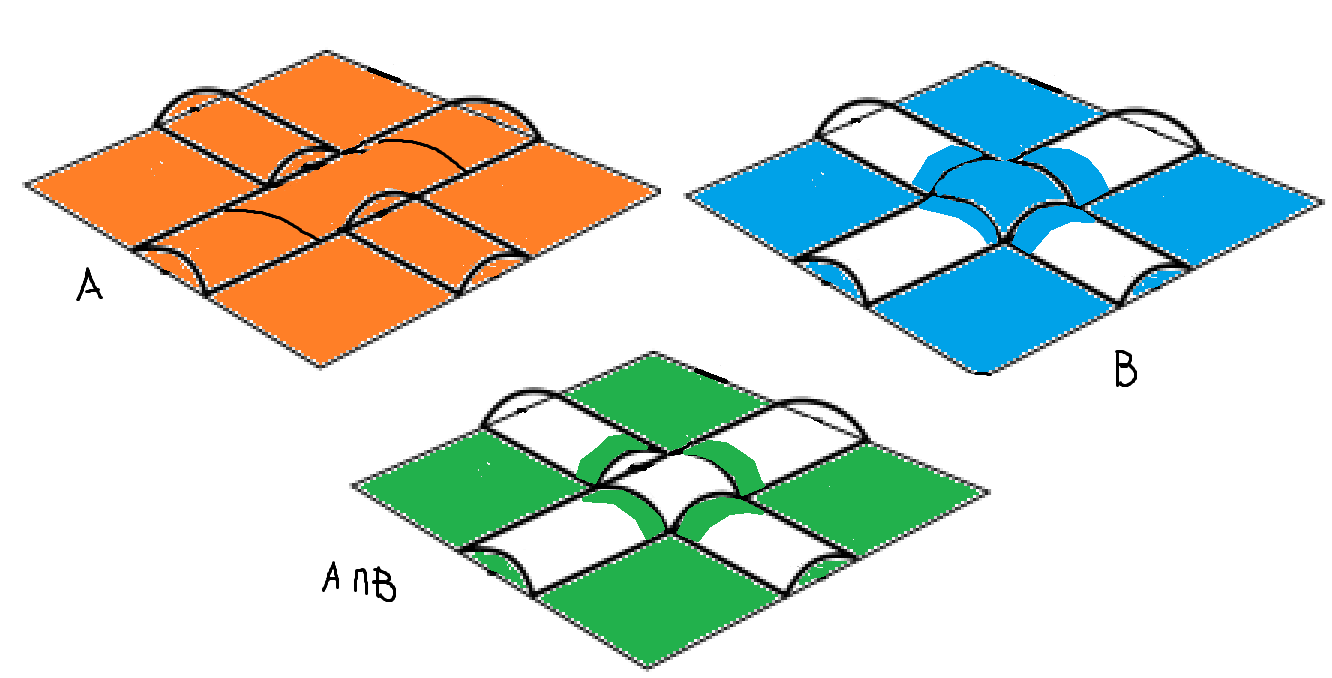
\includegraphics[width=\linewidth]{knot1}
\end{figure}

Pick a basepoint $p$ in $T$. Then, $A$ consists of taking $T$ (which is contractible) and adding a bunch of `thick loops', so it is homotopically equivalent to a wedge of circles, with one circle per arc $\alpha_i$. Thus, its fundamental group is free with one generator, say $x_i$, per arc $\alpha_i$, with this generator going from $p$ to the arc $R_i$ and following it. For the sake of concreteness, \emph{fix an orientation on $K$} (and on $\R^3$), and let $x_i$ follow this loop in the direction given by the right-hand rule, with the thumb following $K$ in the positive direction.

Now, let us look at the fundamental group of $B$. At each crossing, we are (up to homotopy type) appending a square which connects to $T$ via its four corners. By stretching and collapsing stuff, we see that appending a square in this manner is equivalent to wedging with three circles, and so for each crossing the fundamental group of $B$ has three free generators, represented in the following figure. (Not shown in the figure: the paths going from $p$ to the start and end of the pictured loops.)
\begin{figure}[H]
\centering
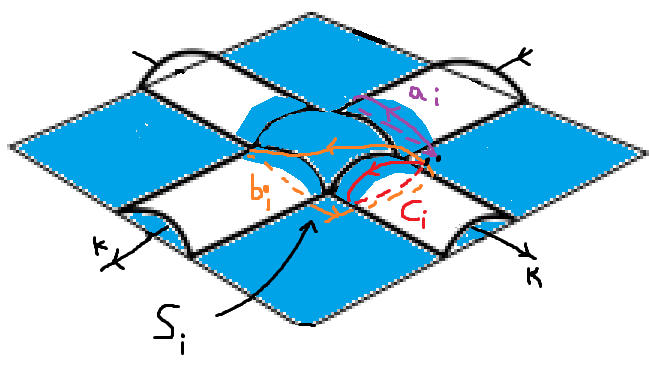
\includegraphics{knot2}
\end{figure}
Note that the orientation of $K$ is pictured in the figure. The convention being followed is that paths are always going around the loop following the right-hand rule.

Finally, we inspect the fundamental group of $A \cap B$. At each crossing we are appending four handles, so the fundamental group of the intersection is free with four generators for each crossing. They are represented in the following figure.
\begin{figure}[H]
\centering
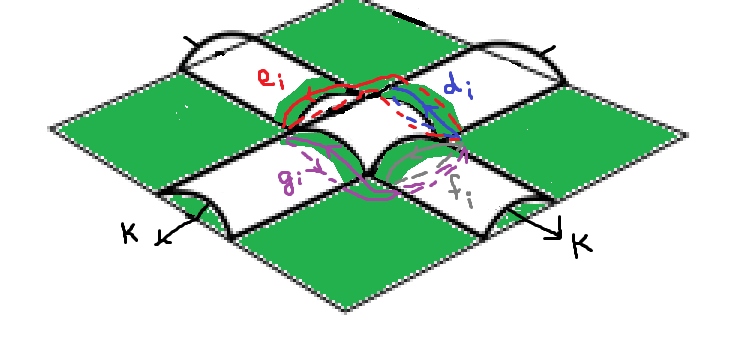
\includegraphics{knot3}
\end{figure}

Finally, we are ready to present the fundamental group of the complement of $K$. To do so, we apply van Kampen's theorem. Note that all spaces involved ($A$, $B$, and $A \cap B$) are path connected because they consist of the tabletop $T \cong \R^2$ with some appendages attached.

The presentation given to us by van Kampen is as follows. We have one generator $x_i$ for each loop, and three generators $a_i$, $b_i$, and $c_i$ for each crossing. Moreover, we have four relations for each crossing, given by $d_i$, $e_i$, $f_i$, and $g_i$.

We will simplify this presentation by inspection. In the following, let $\ell$ be the name of a certain crossing, let $i$ be the name of the arc passing under the crossing, $j$ the arc `going into the crossing' and $k$ the arc `coming out of the crossing'.

The relation given by $d_\ell$ is that $x_i = a_\ell$. This shows that the generators $a_\ell$ are redundant.

The relation given by $f_\ell$ is that $c_\ell = x_k$. This shows that the generators $c_\ell$ are redundant.

The generator $g_\ell$ evidently corresponds to $x_i$ in $A$. It is a little harder to see what it corresponds to in $B$, but inspection will show that $g_\ell = c_\ell^{-1} b_\ell$. Thus, $b_\ell = c_\ell x_i = x_k x_i$. Hence, $b_\ell$ is also redundant.

We are very close to our goal! We have shown that our presentation needs only the generators $x_i$, and we have one relation per crossing, given by $e_\ell$. We now inspect it.

From the perspective of $A$, $e_\ell$ is evidently $x_j$. From the perspective of $B$, a bit of mental gymnastics (deform $b_\ell$ `upwards') will show that $e_\ell = a_\ell^{-1} b_\ell$, and thus we have the relation
\begin{equation}
x_j = x_i^{-1} x_k x_i.
\end{equation}

Solving for $x_k$ we obtain the desired relation. This computes the proof that the fundamental group of the complement of a knot has the presentation we sought.

\item Upon abelianizing, the relations $x_i x_j x_i^{-1} = x_k$ become $x_j = x_k$. Thus, we can show that all $x_i$ are the same as follows. Start at some arc $\alpha_i$, to which corresponds a generator $x_i$. Then, follow along the knot in some direction until the arc ends. This means that you've run into a crossing and that $\alpha_i$ is `jumping over' some arc to become, say, $\alpha_j$. Now, the one relation we have on this crossing tells us that $x_i = x_j$. Now continue to get that $x_j$ equals whatever other generator comes next, and so on. After you've performed a full revolution, you have a chain of equalities between all the generators (this uses the fact that the knot is connected).

At the end, we end up with a group with exactly one generator and no relations, i.e. $\Z$. 
\end{enumerate}
\end{sol}

\begin{ex}[1.3:1]
Let $p \colon \tilde X \to X$ be a covering space, $A \subseteq X$. Show that the restriction of $p$ to $\tilde A = p^{-1}(A)$ is a covering space.
\end{ex}

\begin{sol}
We show this directly. I mean, obviously $p$ is continuous by definition of subspace topology on $\tilde A$. So all that remains to show is that every point has a uniformly covered neighborhood.

Pick $a \in A$. Pick a uniformly covered neighborhood of $a$ in $X$, call it $U$, and set $V = U \cap A$. By definition, $V$ is open in $A$. We claim that $V$ is evenly covered in $A$.

Write $p^{-1}(U) = \coprod W_\alpha$. Then, $p^{-1}(V) = \coprod (W_\alpha \cap \tilde A)$; it is evident that this is a disjoint union.

Finally, since $p$ is a homomorphism restricted to $W_\alpha$, it restricts to a homomorphism restricted to $W_\alpha \cap \tilde A$. We prove this claim now:
\begin{itemize}
\item Injectivity is obvious.
\item Surjectivity: given $v \in V$, it is $p(w)$ for some $w \in W_\alpha$, and evidently $w \in \tilde A$ as well.
\item Continuity: Restricting continuous functions to subspaces preserves continuity.
\item Openness: Perform the above argument for $p^{-1}$.
\end{itemize}

This completes the proof that $p$ restricted to $\tilde A$ is a covering space of $A$.
\end{sol}

\begin{ex}[1.3:6]
Construct a two-sheeted covering space $Y \to \tilde X$ such that the composition $Y \to X$ is not a covering space.
\end{ex}

\begin{sol}
Consider the space $Y$ and map $g$ in the following picture.
\begin{figure}[H]
\centering
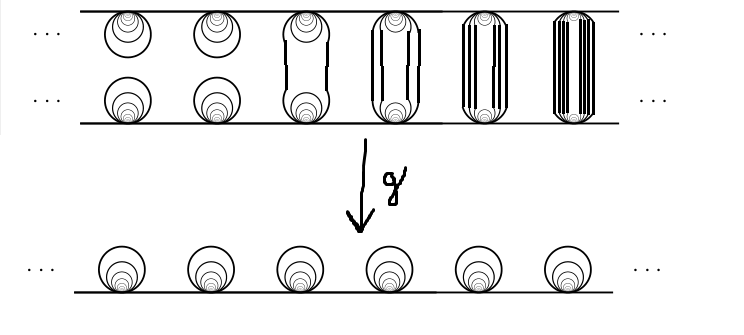
\includegraphics[width=\linewidth]{rings1}
\end{figure}

To the left, we just have infinitely many copies of the hawaiian rings, which are mapped in the obvious way to the rings below them on the picture. Likewise, the two `base lines' are both mapped to the base line below.

Then, on the right, we have `intertwined hawaiian rings', with the number of rings which connect to the opposite basepoint increasing by $1$ with each step to the left.

First, we claim that $g$ is a covering map. Indeed, for the vast majority of points, finding an evenly covered neighborhood is trivial. Indeed, if you remove the points where the circles are all bunched up, topologically both spaces are just a union of countably many copies of an open line segment, and $g$ simply indentifies these lines pairwise. This is obviously a covering map, and since the subspaces in question are open subspaces of $\tilde X$ and $Y$, every such point of $\tilde X$ is evenly covered. It remains to verify that the points of $\tilde X$ at the bunched up circles also have evenly covered neighborhoods.

To do so, consider a fixed such point as in the below figure.
\begin{figure}[H]
\centering
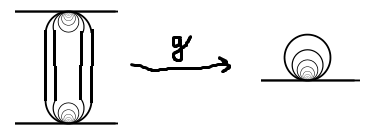
\includegraphics[width=0.7\linewidth]{rings2}
\end{figure}

Then, build a small enough neighborhood of this point which encompasses only partially the rings which, in $Y$, are connected to another basepoint. Then, it is easy to see that such a neighborhood is evenly covered (twice); see figure below.
\begin{figure}[H]
\centering
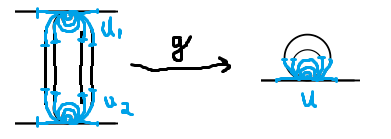
\includegraphics[width=0.8\linewidth]{rings3}
\end{figure}

Now, let us show that the composite $f \circ g$, where $f$ is the map $\tilde X \to X$, is not a covering map. The problem is going to be at the point of $X$ where all the circles are bunched up, call it $p$.

Suppose that there is some evenly covered neighborhood $U$ of $p$. We remark on the following fact about the hawaiian rings: \emph{any neighborhood $U$ of $p$ will contain infinitely many rings in their entirety.}

Now, consider $(f \circ g)^{-1}(U)$. We will show that this is not a union of disjoint sets all of which are homeomorphic to $U$ by $p$. To do so, pick some ring $r$ which is entirely contained in $U$. Then, go far enough to the right in $Y$ that this ring becomes a segment between two distinct basepoints. Thus, you may find a path between two distinct points in $(f \circ g)^{-1}(p)$ which is contained in $(f \circ g)^{-1}(U)$. Of course, this is a contradiction, because such a thing cannot happen in an evenly covered neighborhood. (By taking the preimages of the $U_\alpha$ you would obtain a contradiction with the connectedness of the interval.) Thus, the exercise is complete.
\end{sol}

\begin{ex}[1.3:10]
Find all connected $2$-sheeted and $3$-sheeted covering spaces of $S^1 \vee S^1$, up to isomorphism without basepoint.
\end{ex}

\begin{sol}
We do this process geometrically, starting with the $2$-sheeted covers. We know that $S^1 \vee S^1$ is a graph, and therefore so is any of its covering spaces, with vertices in the cover corresponding to vertices in the base space and likewise for edges. Moreover, two sheetedness means that the number of edges and vertices are doubled, so we have two vertices and four edges to `distribute between the vertices'.

For the sake of definiteness, let the two (oriented) edges of $S^1 \vee S^1$ be labeled $a$ and $b$. Then, in the covering space, there are two (oriented) edges also labeled $a$ and $b$. Since the graph is connected, there must be an edge going from one of the vertices to the other. Without loss of generality, we suppose that it is an $a$ edge; at the end we may obtain the missing covering spaces by swapping $a$ and $b$. Now, both vertices look locally like the vertex of $S^1 \vee S^1$, so they must both have one $a$ going in and one $a$ going out (and likewise for $b$). Hence, the one $a$ edge we have determines the other, so so far our covering space looks like this.
\begin{figure}[H]
\centering
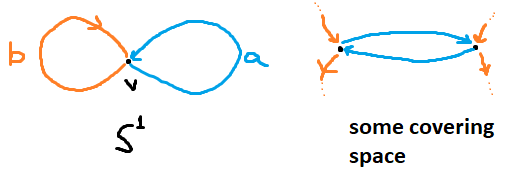
\includegraphics{cov1}
\end{figure}

Now, all that remains is to complete the $b$ edges. There are evidently two, and only two, possible arrangements. Taking those two arrangements and taking the symmetric wrt $a$ and $b$, we obtain a total of three two-sheeted connected coverings of $S^1 \vee S^1$, pictured below.
\begin{figure}[H]
\centering
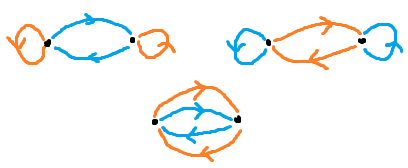
\includegraphics{cov2}
\end{figure}

Note: All of these are distinct because they correspond to distinct subgroups of $\braket{a,b} = \pi(S^1, v)$, respectively (from left to right): $\braket{b,a^2, aba^{-1}}$, $\braket{a,b^2,bab^{-1}}$, and $\braket{a^2, b^2, ab}$. These can be distinguished by querying whether $a$ and $b$ are in each group, arguing by parity that e.g. neither is in the last subgroup.

\medskip

Let us move on to three-sheeted coverings. Arguing as above, there must be three vertices and three copies of each edge. Let us call the vertices $1$, $2$, and $3$. By connectedness, there must be an edge (suppose $a$ as above) going from (without loss of generality) $1$ to $2$. On the other hand, there must be an outgoing edge $a$ from $2$, which cannot return to $2$ because it already has an incoming $a$. This edge must hence go to $1$ or $3$, so any covering looks partially like one of the following two.
\begin{figure}[H]
\centering
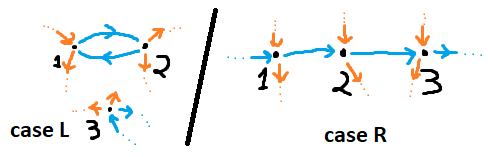
\includegraphics[width=\linewidth]{cov3}
\end{figure}

Of course, it is evident that the third $a$ edge is determined, so it suffices to inspect the $b$ edges now.

On the left case (case L), by connectedness, the $b$ edges of $3$ must connect to $1$ or $2$. Without loss of generality, by symmetry, suppose the outgoing edge is $b \colon 3 \to 1$, so the question is whether the other edge is $1 \to 3$ or $2 \to 3$. As it happens, this choice determines the covering, and the possible outcomes are displayed in the following figure.
\begin{figure}[H]
\centering
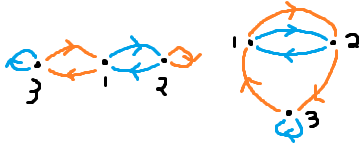
\includegraphics[width=\linewidth]{cov4}
\end{figure}

Now, let us inspect case $R$. In this case, the $a$ edges form a loop. Moreover, we may assume without loss of generality that the $b$ edges do not have the same structure as the $a$ edges do in case $L$ (because we will already have those cases covered when we swap $a$ and $b$). Thus, we assume that either the $b$ edges have no self-loops (i.e. they are always from and to distinct vertices) or that they have more than one self-loop (in which case they must all be self-loops). In the case where there are no self-loops, the $b$ edges form a cycle, which may have the same orientation as the $a$ loop or opposite. Thus, we obtain the following three cases for case $R$.
\begin{figure}[H]
\centering
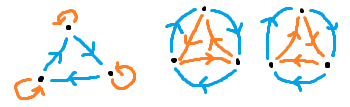
\includegraphics[width=\linewidth]{cov5}
\end{figure}

We conclude this exercise thus: The classification of three-sheeted coverings of $S^1 \vee S^1$ is given by the five coverings above outlined, as well as their `$a$-$b$ mirrors', in the sense of replacing $a$ edges with $b$ and vicer versa. Some of these coverings are symmetric, so we obtain only 7 coverings at the end. The following picture displays these coverings as well as some subgroups of $\braket{a,b}$ they correspond to, until I got bored. Then I just wrote why I'm sure they are distinct: evidently the Galois covers are different from non-Galois, and inside each group I wrote some property of the corresponding subgroup of $\pi(S^1 \vee S^1, v)$ which lets us distinguish this cover from others.
\begin{figure}[H]
\centering
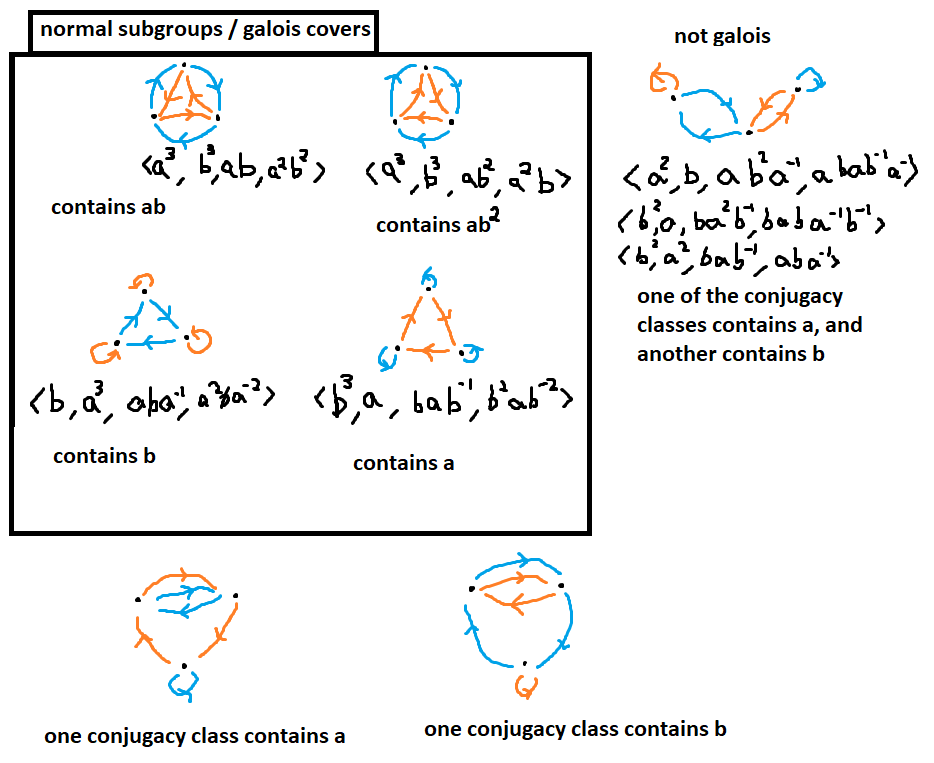
\includegraphics[width=\linewidth]{cov6}
\end{figure}
\end{sol}

\begin{ex}[1.3:13]
Determine the covering space of $S^1 \vee S^1$ which corresponds to the subgroup of $\pi(S^1 \vee S^1)$ generated by the cubes of all elements.
\end{ex}

\begin{sol}
As proposed by the problem statement, we represent this covering space, which we call $S$, as a graph embedded in the torus. We use the same pictorial notation for the covering as in the previous exercise. Note that this torus is not a rectangle with edges identified, but rather two glued equilateral triangles.
\begin{figure}[H]
\centering
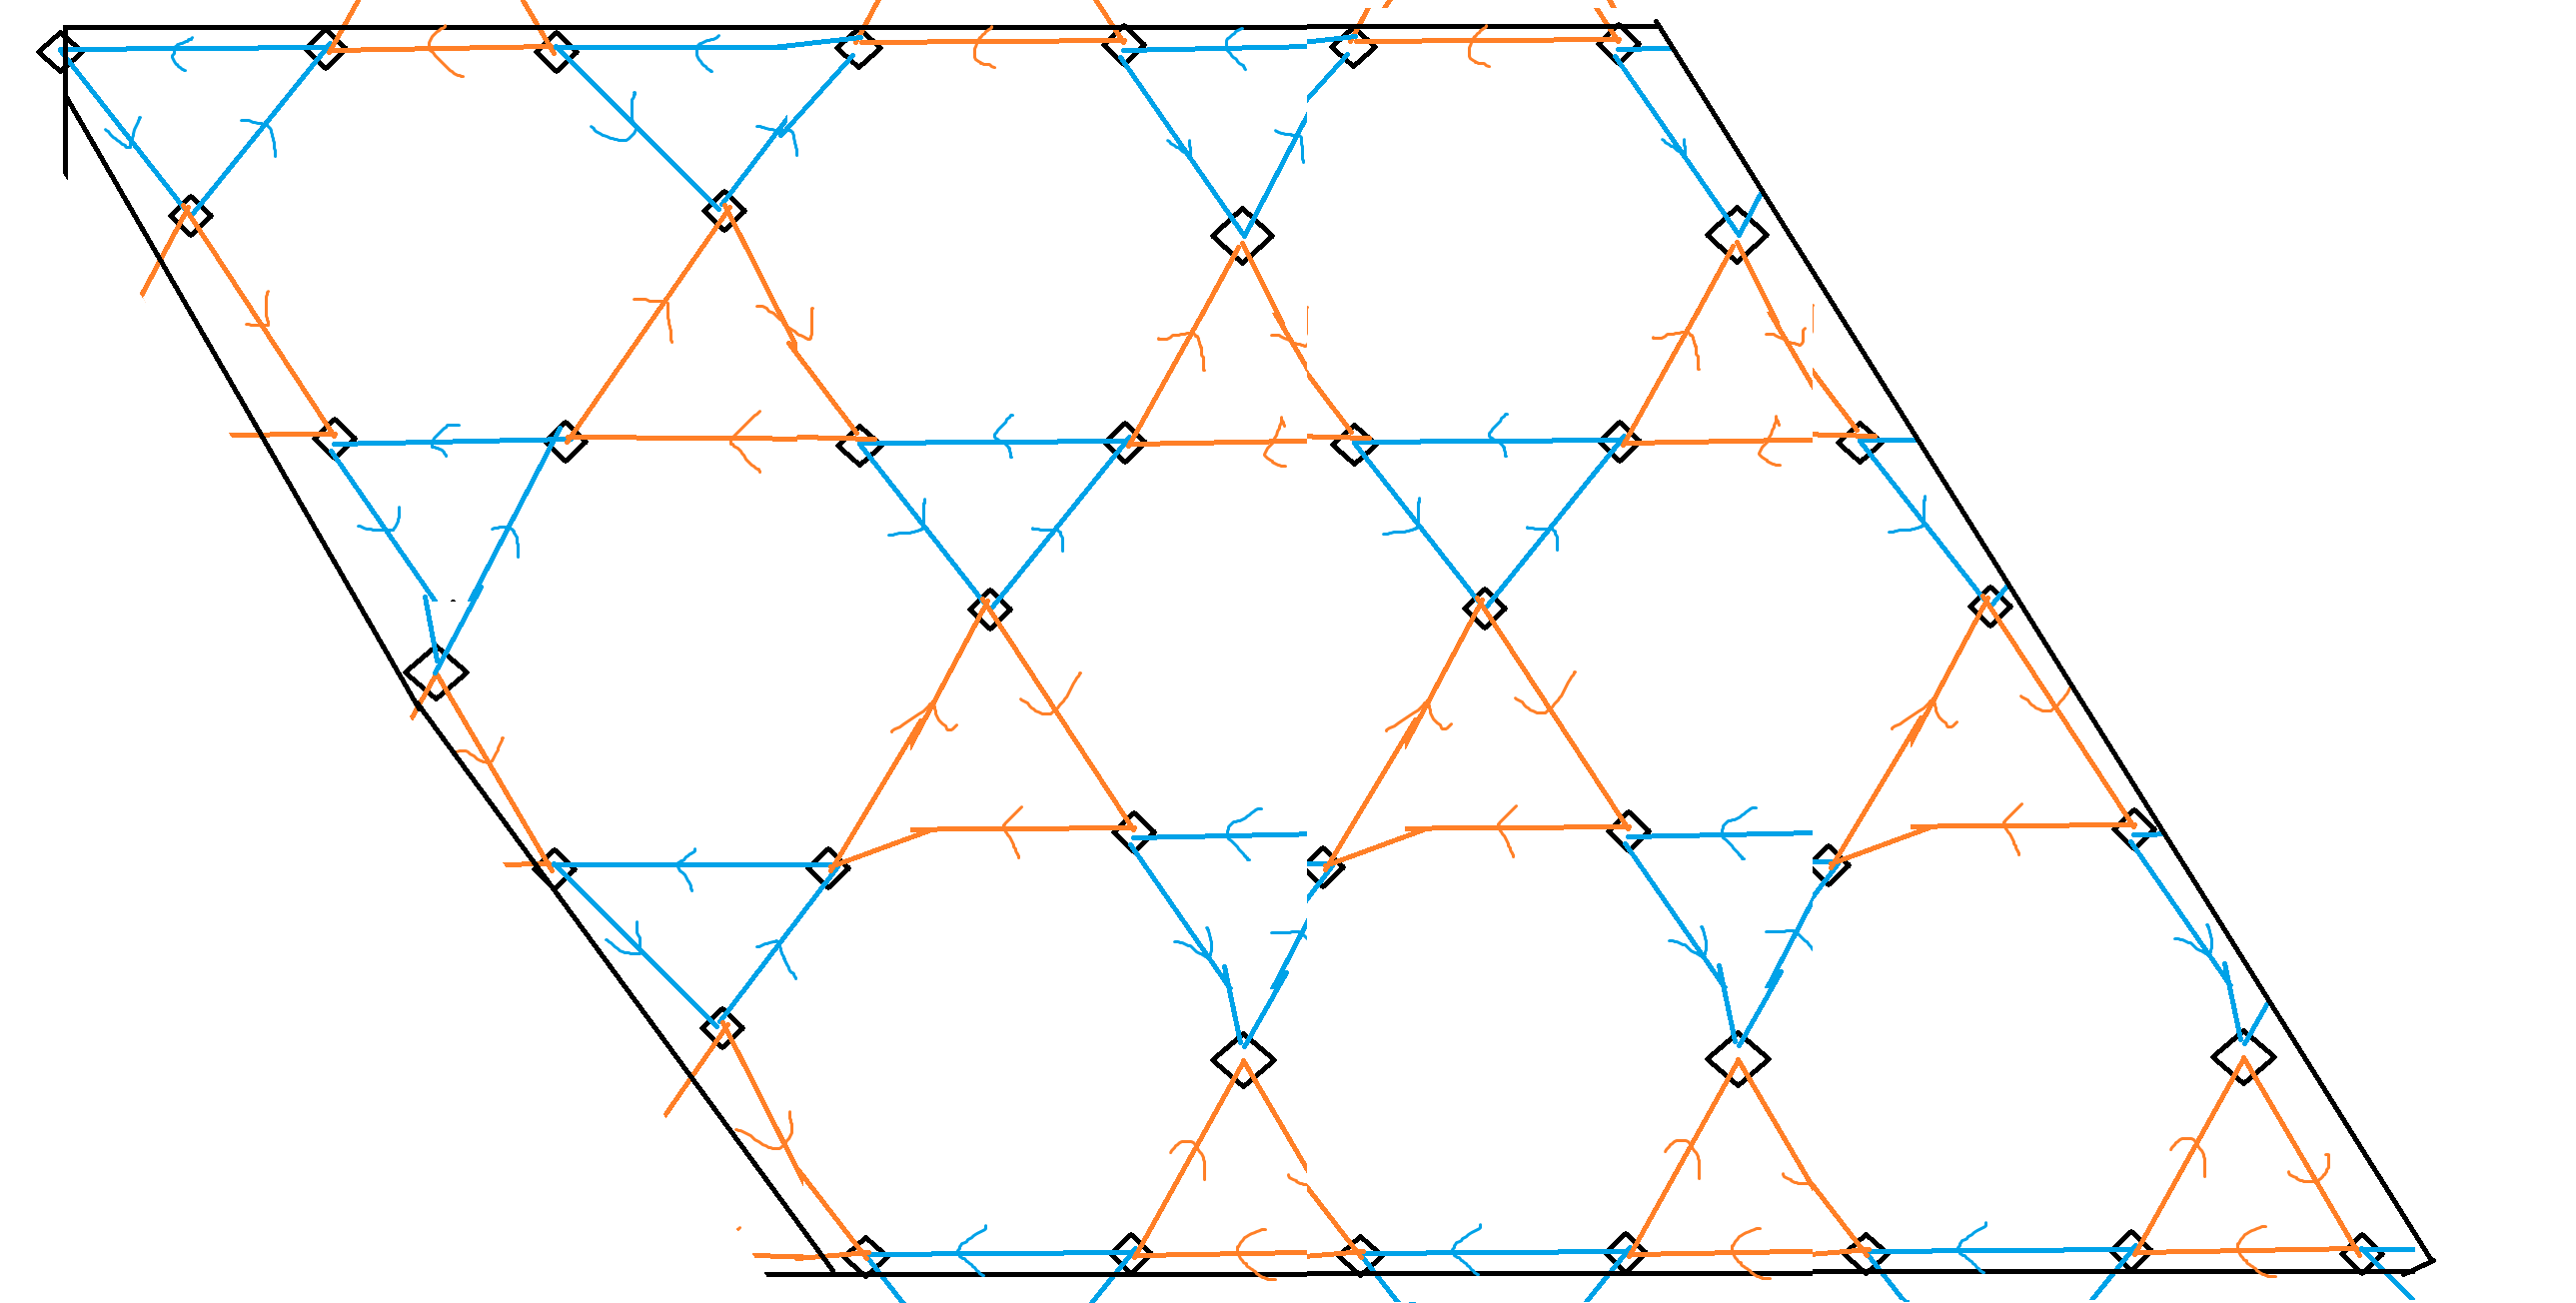
\includegraphics[width=\linewidth]{cov7}
\end{figure}

We will now show that this covering space $S$ does correspond to the subgroup generated by all cubes. Let $G_1$ be the subgroup of $\braket{a,b}$ that corresponds to the covering space above (pick some basepoint, it doesn't really matter which), and let $H$ be the subgroup of $\braket{a,b}$ generated by all cubes. We intend to show that $G_1 = H$.

First, let us show that $G_1 \subseteq H$. To do so, we note that $G_1$ is a finite graph, and hence its free group is a free group in some number of generators. If we can find such a set of generators, we can easily verify individually that each of them is in $H$. To do so, the first step is to pick a spanning tree; then, each edge not in the tree represents a generator (given by following the tree to one of the vertices, going through the edge, and then following the tree to the basepoint). Thus, we begin by picking a spaning tree; it is purple in the figure below. In red, we point out and number the edges which correspond to generators.
\begin{figure}[H]
\centering
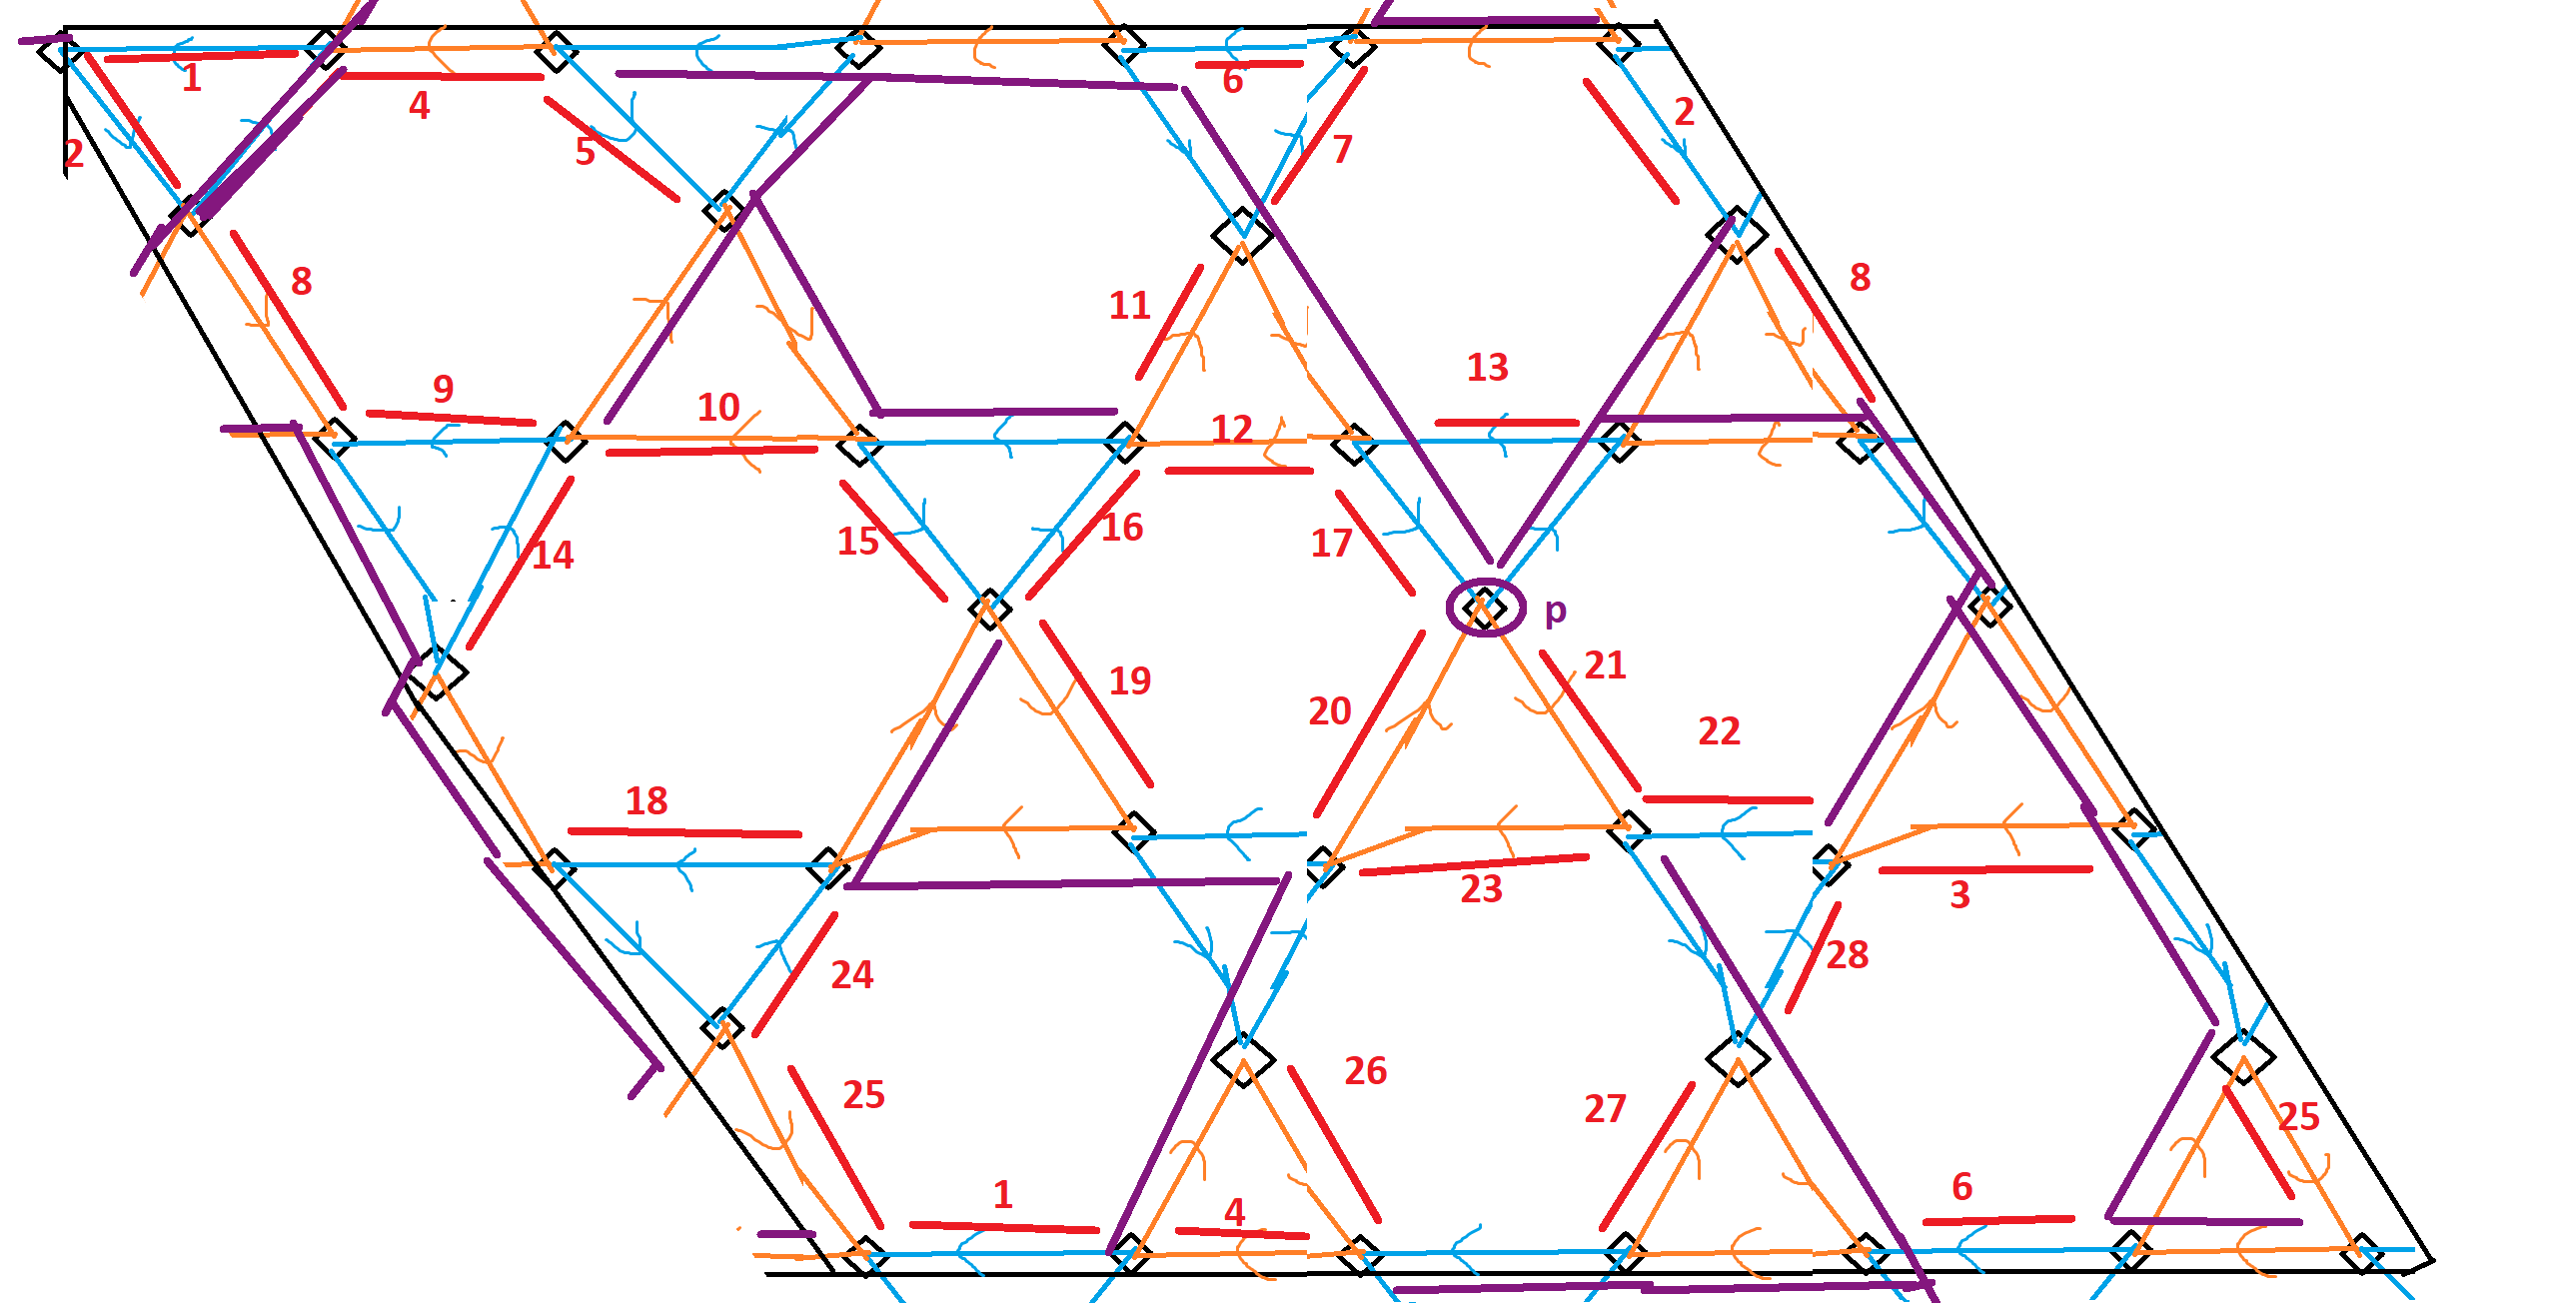
\includegraphics[width=\linewidth]{cov82}
\end{figure}

Now, we simply manually check, for each of these edges, what element of $G_1$ they correspond to, and verify that such an element is in $H$ by writing it as the cube of something. We do so in the following table.
\begin{center}
\setlength\extrarowheight{0.6ex}
\[
\begin{array}{c | c | c}
\text{Edge} & \text{Generator} & \text{In $H$ because equals} \\
\hline
\hline
1 & aba(a)b^2 a^{-1} b^{-1} a^{-1} b a^{-1} & ab \left[ [a^{-1} (a^3 b^3 (b^{-1} a^{-1})^3) a] b^3 \right] (ab)^{-1} \\
\hline
2 & ab (a^{-1}) b^2 a^{-1} b^{-1} a^{-1} b a^{-1} & ab \left[ [a^{-1} (b^3 (b^{-1} a^{-1})^3) a] b^3 \right] (ab)^{-1} \\
\hline
3 & ab^{-1} a b^{-1} (b^{-1}) b^{-1} a^{-1} b a^{-1} & (a b^{-1} a) (b^{-1})^3 (a b^{-1} a)^{-1} \\
\hline
4 & a b a (b^{-1}) a^{-1} b^{-1} a b a & aba (b^{-1} a^{-1})^3 (aba)^{-1} (aba)^3 \\
\hline
5 & a^{-1} b^{-1} a^{-1} b a (a) a b^{-1} a b a & (a^{-1} b^{-1} a^{-1} b) a^3 (a^{-1} b^{-1} a^{-1} b)^{-1} \\
\hline
6 & a^{-1} b^{-1} a^{-1} (a^{-1}) b a^{-1} b^{-1} a^{-1} b a^{-1} & ???
\end{array}
\]
\end{center}

Ok so I lost patience to finish this table. But assuming the statement is true, after enough time I would have a finished and correct table which would prove the statement I'm trying to show. Maybe it would be nicer with a more well chosen spanning tree but none stood out as simplifying the problem drastically. Now I am bored so I'll just pretend that this part of the solution is done and move on to the second part of the proof.

\smallskip

Now, let us show that $H \subseteq G_1$. It suffices to show that all generators of $H$ are in $G_1$. So, consider some generator of the form $x^3$. We will show that the deck action of $x^3$ on the basepoint of $S$ is null (which shows that $x^3$ is in $G_1$).

We do case checking based on where a chosen basepoint $p$ of $S$ goes after the action of $x$. Suppose for the sake of argument that $p$ is the bottom vertex of a blue triangle. Then, after the action of $x$, $p$ may or may not be the bottom vertex of a blue triangle. If it is not, then it is easy to check that the displacement from $xp$ to $x^2 p$ is a $\pm 120^\circ$ degree rotation of the displacement from $p$ to $xp$ (Proof sketch: Induct on the length of the word $y \in \braket{a,b}$ to show that the displacement $q$ to $yq$ is a rotation of the displacement from $p$ to $yp$, where $q$ is a non-bottom vertex of a blue triangle), and the same holds for the displacement from $x^2 p$ to $x^3 p$ rel the displacement $xp$ to $x^2 p$, so the displacement from $p$ to $x^3 p$ is a sum of a vector with its two $180^\circ$ rotations, which is null. Hence, the deck action of $x^3$ is null, and so $x^3 \in G_1$.

On the other hand, we can also show by induction on the length of $y$ that if $p$ and $q$ are both lower vertices of a triangle, the displacement between $p$ and $yp$ is the same as the one between $q$ and $yq$. Thus, the displacement between $p$ and $x^3 p$ is thrice the displacement between $p$ and $xp$. Now, a bit of case checking (there's nine cases, which is easily reduced to four) will show that the displacement between any two bottom vertices of blue triangles, when tripled, is null in the torus. Thus, $p = x^3 p$.

This concludes the proof that the deck action of $x^3$ on the basepoint of $S$ is always null, and therefore that the action itself is null, hence that $x^3 \in G_1$, and by arbitraryness of $x$ that $H \subseteq G_1$. Therefore, $H = G_1$ and thus $S$ is the covering space that corresponds to $H$.
\end{sol}

\begin{ex}[1.3:31]
Show that the normal covering spaces of the wedge of $n$ circles are the Cayley graphs of groups with $n$ generators.
\end{ex}

\begin{sol}
Let $X$ be the wedge of $n$ circles, and let $p \colon \tilde X \to X$ be a normal covering. Let $G = \pi(X, *)$ where $*$ is the basepoint of $X$, and $H$ be the subgroup of $G$ that $\tilde X$ corresponds to. There is no ambiguity in this statement because $H$ is normal and thus invariant under conjugation/change of basepoint in $\tilde X$.

We know that the group of deck transformations of $\tilde X$ is canonically isomorphic to $G / H$. Moreover, if we fix a basepoint $e \in \tilde X$, there is a canonical bijection between $G/H$ and $p^{-1}(*)$, given by $[g] \mapsto g \cdot e$. We will show that in fact $\tilde X$ is the Cayley graph of $G/H$, with the generating set being the (projections of the) (canonical) generators of $G$.

Indeed, given an edge from $g \cdot e$ to $h \cdot e$, we know that this edge corresponds to an edge of $X$, and thus to a generator $a$ of $G$ (or its inverse). It is obvious by definition that $a \cdot (g \cdot e) = h \cdot e$, and hence that $h = ga$ (ah crap why am I writing a right action with left action notation. Sorry.) Therefore, \emph{every edge in the graph corresponds to a generator of $G$, and it goes from the element corresponding to $q \in G/H$ to $[a] q$}, where $a$ is a generator of $G$.

On the other hand, it is obvious that given a vertex, any generator of $G$ corresponds to an edge of this vertex.

In conclusion, any normal covering $\tilde X$ corresponds to a Cayley graph in $n$ generators. We now turn to showing the converse.

\smallskip

Let $Q$ be a group in $n$ generators, and let $\tilde X$ be its Cayley graph. Now, define $p \colon \tilde X \to X$ as follows: all vertices are taken to $* \in X$, edges corresponding to generators are taken to the corresponding circle in $X$ [assuming we've previously assigned each generator of $Q$ to a circle in $X$], and edges corresponding to inverses of generators are taken to the corresponding circles, but backwards.

This is a covering space. Indeed, we may find an evenly covered neighborhood of any point in $X$ manually, by separating $X$ into `basepoint' and `not the basepoint' and doing separate but obvious constructions accordingly.

Finally, we need to show that it is a normal covering space. To do so, we show that the subgroup it corresponds to is the kernel of the obvious map $f$ from $\pi(X,*)$, i.e. the free group in $n$ generators, to $Q$. Indeed, an element of the kernel is a word in $n$ generators which, when followed in the graph $\tilde X$, goes from the identity to the identity. Thus, it corresponds to a loop in $\tilde X$, and thus to an element of the subgroup of $\pi(X,*)$ corresponding to $\tilde X$. On the other hand, an element of the subgroup of $\pi(X,*)$ corresponding to $\tilde X$ is a word in $n$ generators which, when followed in $\tilde X$, becomes a loop, and therefore goes from the identity to the identity. Hence, by definition of the Cayley graph, $f$ of this is null, and thus it is in the kernel of $f$.

This completes the correspondence between normal coverings of $X$ and Cayley graphs in $n$ generators.
\end{sol}

\end{document}